\chapter{Output Reports}
\label{app:outputReports}
Motea sets the report mode to 0x35 as soon as the connection to the Wii remote is established. This is done by sending the following bytes to the Wii remote:
\begin{quote}
0xA2 0x12 0x04 0x35
\end{quote}
The first byte indicates that it is an output report, the second byte is the ID of the report type, the third byte indicates whether to use continuous reporting (send report even when there has been no change to the data) and the fourth indicates which report mode to set. The report mode has to be set again whenever an extension is discovered, this can be detected by the fact that you receive a status information report without requesting one. In such cases Motea immediately sends a request to set the report mode to 0x35.

Report mode 0x35 contains core button (0xbb), acceleromter (0xaa), and extension data (0xee):
\begin{quote}
0xA1 0x35 0xbb 0xbb 0xaa 0xaa 0xaa 0xee 0xee 0xee 0xee ... (16 bytes of type 0xee)
\end{quote}

The LEDs on the Wii remote can be controlled by using output report 0x11:
\begin{quote}
0xA2 0x11 0x80
\end{quote}
The third byte indicates which lights to turn on, the four most significant bits of this byte each represents one LED (in the example above the rightmost byte is enabled):
\begin{quote}
0b0000 0000 : no lights\\
0b1000 0000 : rightmost LED enabled\\
0b1100 0000 : the two rightmost LEDs enabled\\
etc.
\end{quote}
Motea also uses this report mode to initialize the rumble pack. The least significant bit of the third byte of any output report turns sets the status of the rumble pack, where 1 is on and 0 is off. As an example, let us say we have the two rightmost LEDs activated and the rumble pack is to be turned on, the report would look like this:
\begin{quote}	
0xA2 0x11 0xC1\\
(0xC1 = 0b1100 0001 the least significant bit representing the rumble pack)
\end{quote}
As previously stated all output reports have to change the least significant bit of the third byte to one if the rumble pack is to stay active. Therefore Motea has to keep track of the state of the rumble pack and change the output reports accordingly. All examples in this section, other than the one above, will assume that rumbling is turned off.

Status information can be requested by sending:
\begin{quote}
0xA2 0x15 0x00
\end{quote}
A status information report with ID 0x20 is then sent from the Wii remote to the host:
\begin{quote}
0xA1 0x20 0xbb 0xbb 0xss 0x00 0x00 0xll
\end{quote}
0xbb (bytes 3 and 4) contains data about the core buttons. 0xss contains data about which LEDs are enabled and whether the following features are enabled: speaker, extension controller, and continouous reporting. 0xll holds the battery level. 

Writing to registers is done by sending:
\begin{quote}
0xA2 0x16 0x04 0xaa 0xaa 0xaa 0xll 0xdd 0xdd ...
\end{quote}
Here 0xaa (bytes 4-6) represents the register address to write to. 0xll is the number of bytes to write. 0xdd (bytes 8-) is the data to be written to the register, usually only one byte is written.

Reading from registers/memory is done by sending:
\begin{quote}
0xA2 0x17 0xmm 0xaa 0xaa 0xaa 0xll 0xll
\end{quote}
0xmm sets whether to read from memory or from the registers, in motea only the calibration report for the accelerometer is read from memory. 0xaa (bytes 4-6) is the address to read from. 0xll (bytes 7 and 8) is the length of data to be read. After a read request is sendt the Wii remote sends the data in return using a report with ID 0x21:
\begin{quote}
0xA1 0x21 0xbb 0xbb 0xse 0xaa 0xaa 0xdd 0xdd ... (16 bytes of the type 0xdd)
\end{quote}
0xb (byte 3-4) is core button data. 0xse holds both the size of the data returned and the error flag. 0xdd (bytes 8-23) contain the requested data (as long as there was no error).

\chapter{MotionPlus}
\label{app:gyroParse}

When you plug in a normal extension to the Wii remote it is automatically receive a status information report notifying that an extension has been connected. Pluging in the MotionPlus however, will not result in such a status information report. To check if the MotionPlus extension is pluged in, the two bytes from Wii remote register address 0xA600FE has to be read by sending the read request:
\begin{quote}
0xA2 0x17 0x04 0xA6 0x00 0xFE 0x00 0x02
\end{quote}
After sending this request a data report with ID 0x21 is sent in return containing the requested data. The received data report contains the two bytes read from register 0xA600FE. The meaning of these bytes are shown in table~\ref{tab:motionPlusStatus}. If the MotionPlus extension is not connected the data report will fail with error 7.
\begin{table}[h!]
\begin{tabularx}{\textwidth}{|l|X|}
\hline
Value  & Meaning \\ \hline
0x0005 & MotionPlus is pluged in, but not initialized \\ \hline
0x0405 & No longer active MotionPlus\\ 
\hline
\end{tabularx}
\caption{\footnotesize MotionPlus status}
\label{tab:motionPlusStatus}
\end{table}

After confirming that the MotionPlus extension is pluged in, the next thing to do is to initialize it. This is done by writing 0x55 to 0xA600F0, by sending the following report:
\begin{quote}
0xA2 0x16 0x04 0xA6 0x00 0xF0 0x01 0x55
\end{quote}

When the MotionPlus has been initialized it has to be activated before we can receive data from it. This is done by writing 0x04 to register address 0xA6 0x00 0xFE:
\begin{quote}
0xA2 0x16 0x04 0xA6 0x00 0xFE 0x01 0x04
\end{quote}
After the MotionPlus extension has been activated the Wii remote will send a status information report, informing that an extension has been connected. Now the extension bytes of data report 0x35 will contain gyroscope data form the MotionPlus.

The 32 bytes from register 0xA60020 holds the calibration data for the MotionPlus. According to the WiiBrew wiki \cite{wiiBrew} it is still unclear how they work. However, by looking at the WiiMoteLib \cite{wiiMoteLib} library an implementation using this calibration data was found. Unfortunately this implementation is not very accurate, at least not compared to manual calibration. Aquireing the data is done by sending the read request:
\begin{quote}
0xA2 0x17 0x04 0xA6 0x00 0x20 0x00 0x32
\end{quote}

Extension data is received with every report of ID 0x35:
\begin{quote}
0xA1 0x35 0xbb 0xbb 0xaa 0xaa 0xaa 0xee 0xee 0xee 0xee ... (16 bytes of type 0xee)
\end{quote}
Here 0xbb represents core button data and 0xaa represents acceleration data. The extension data is contained in the 16 last bytes shown by 0xee above. The gyroscope data is contained in the 6 first bytes of the extension data. The data format is shown in figure~\ref{fig:motionPlusDataFormat}. The gyroscope has two modes: fast and slow. These values tells us what type of scaling to use to get the correct degrees per second. According to WiiBrew \cite{wiiBrew} 20 units correspond to 1.45 deg/s in slow mode and 6.59 deg/s in fast mode. Motea uses slightly different values, taken from WiiMoteLib \cite{wiiMoteLib}: 20 units corresponding to 1 deg/s in slow mode and 5 deg/s in fast mode. Which of these values give more accurate data has not been tested, and since the Madgwick algorithm \cite{madgwick} compensates roll and pitch using the acceleromter, a small error in the gyroscope data can be tolerated. 
\begin{figure}[h!]
  \centering
    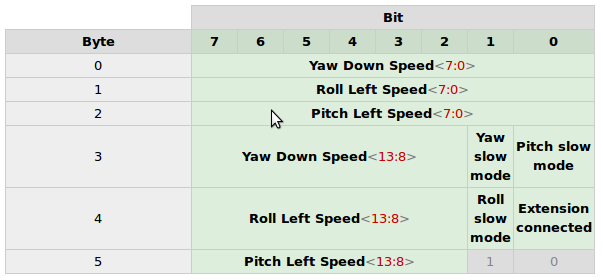
\includegraphics[width=.80\textwidth]{motionPlusDataFormat.png}
    \caption{\footnotesize Motion Plus data gyroscope data format}
    \label{fig:motionPlusDataFormat}
\end{figure}

Motea parsing and calibrating gyroscope data:
\begin{lstlisting}
// Get fast/slow mode
boolean yawFast = ((extensionData[3] & 0x02) >> 1) == 0;
boolean rollFast = ((extensionData[4] & 0x02) >> 1) == 0;
boolean pitchFast = ((extensionData[3] & 0x01) >> 0) == 0;

// Get raw data
float yaw = 
	((extensionData[0] & 0xff) | ((extensionData[3] & 0xfc) << 6));
float roll = 
	((extensionData[1] & 0xff) | ((extensionData[4] & 0xfc) << 6));
float pitch = 
	((extensionData[2] & 0xff) | ((extensionData[5] & 0xfc) << 6));

// Manual calibration
if (!calibration.isFinished()) {
	calibration.addCalibrationData(yaw, roll, pitch);
	if (calibration.isFinished()) {
		calibrationData = calibration.getCalibratedData();
	}
}

// Calibrate raw data
yaw -= calibrationData.getYaw0();
roll -= calibrationData.getRoll0();
pitch -= calibrationData.getPitch0();

// Set scaling
if (yawFast) {
	yaw /= HIGHSPEED_SCALING;
} else {
	yaw /= LOWSPEED_SCALING;
}

if (rollFast) {
	roll /= HIGHSPEED_SCALING;
} else {
	roll /= LOWSPEED_SCALING;
}

if (pitchFast) {
	pitch /= HIGHSPEED_SCALING;
} else {
	pitch /= LOWSPEED_SCALING;
}
\end{lstlisting}